\section{Results}\label{sec:results}
\subsection{BioCLIP on real photos}
Table~\ref{tab:reference} gives the reference: BioCLIP's accuracy on unmodified photos of each real dataset.
\todo{One sentence: e.g. high on inat80, lower on rare, as expected for held-out species.}
\begin{table}[t]\centering\small
\caption{BioCLIP (open set) on real photos.}\label{tab:reference}
\resizebox{\columnwidth}{!}{\begin{tabular}{lrrrr}
\toprule
dataset & n & accuracy & genus_acc & vlm_agrees \\
\midrule
invasive & 320 & 0.322 & 0.488 & 0.803 \\
\bottomrule
\end{tabular}
}
\end{table}

\subsection{Attack success}
\begin{table*}[t]\centering\small
\caption{Attack success per dataset and method (faithful = VLM judge; ASR with 95\% bootstrap CI).}\label{tab:main}
\resizebox{\textwidth}{!}{\begin{tabular}{llrrrrrrrrrr}
\toprule
dataset & method & n & faithful_rate & ASR & ASR_lo & ASR_hi & effective_ASR & effective_ASR_lo & effective_ASR_hi & ASR@family & taxo_dist \\
\midrule
inat80 & img2img & 1920 & 0.697 & 0.510 & 0.438 & 0.585 & 0.356 & 0.305 & 0.407 & 0.239 & 2.701 \\
invasive & img2img & 638 & 0.588 & 0.755 & 0.657 & 0.835 & 0.444 & 0.372 & 0.516 & 0.533 & 3.438 \\
synth80 & baseline & 68 & 0.941 & 0.219 & 0.141 & 0.299 & 0.206 & 0.132 & 0.279 & 0.062 & 2.214 \\
synth80 & llm & 120 & 0.842 & 0.485 & 0.258 & 0.711 & 0.408 & 0.217 & 0.600 & 0.218 & 3.265 \\
synth80 & targeted & 120 & 0.792 & 0.400 & 0.170 & 0.639 & 0.317 & 0.133 & 0.496 & 0.232 & 3.211 \\
synth80 & templates & 80 & 0.775 & 0.371 & 0.175 & 0.594 & 0.288 & 0.138 & 0.482 & 0.177 & 2.870 \\
\bottomrule
\end{tabular}
}
\end{table*}
Table~\ref{tab:main} and Figure~\ref{fig:asr} compare all methods. \todo{Main findings: which family of modifiers
works best (tables/families), how targeted and LLM prompts compare to templates, the gain of best-of-N, the effect of
img2img strength (Figure~\ref{fig:i2i}), and how far in the tree the errors go (Figure~\ref{fig:taxo}).}

\begin{figure}[t]\centering
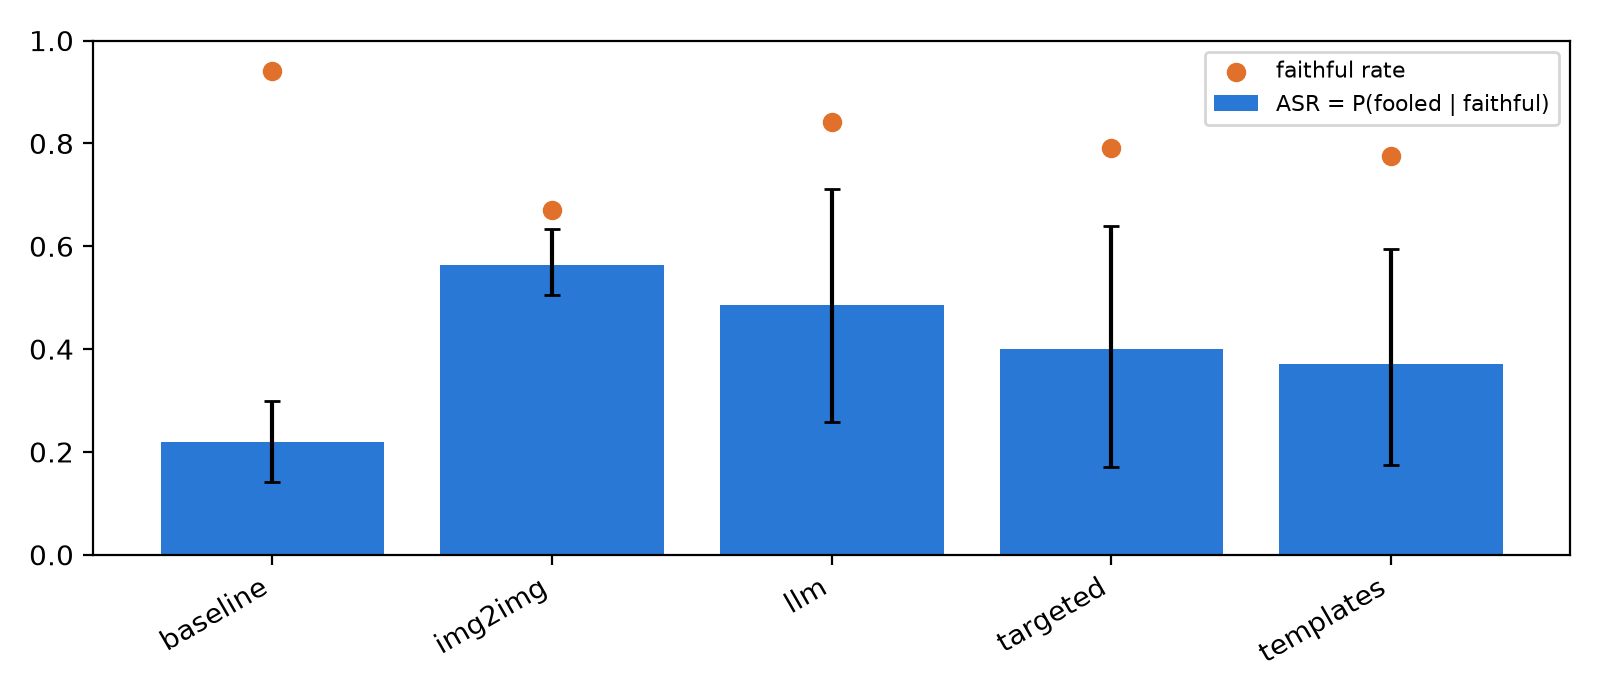
\includegraphics[width=\columnwidth]{../results/figures/asr_by_method.png}
\caption{ASR (bars, 95\% CI) and faithful rate (dots) per method.}\label{fig:asr}
\end{figure}
\begin{figure}[t]\centering
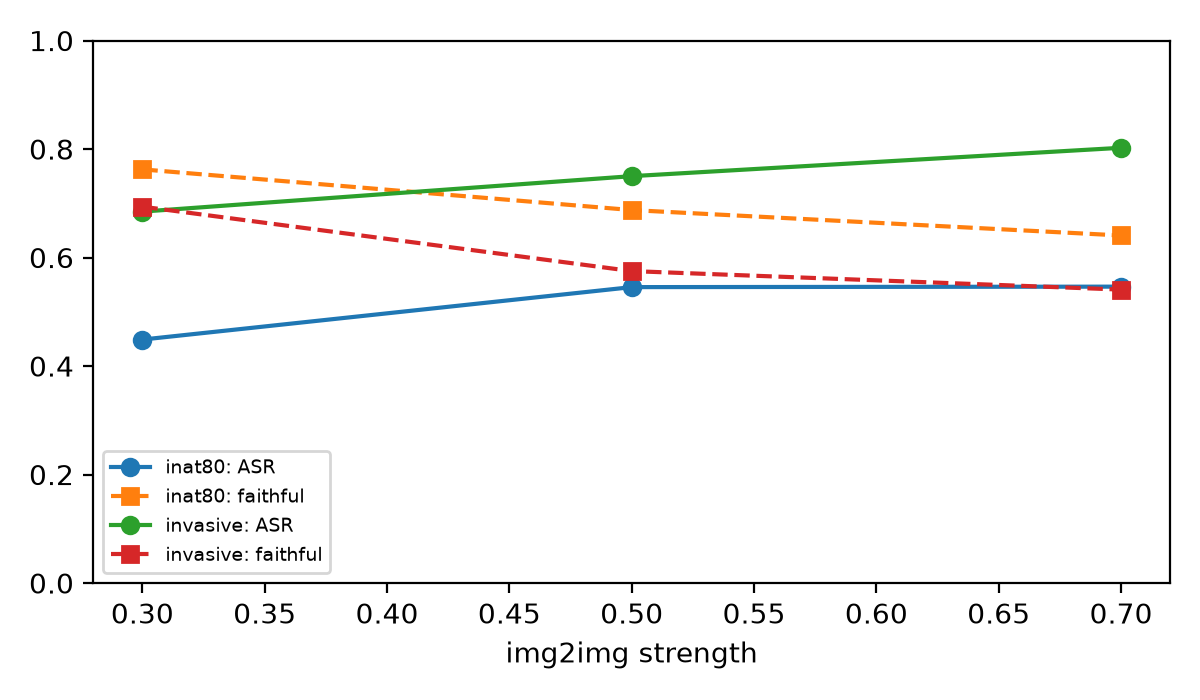
\includegraphics[width=\columnwidth]{../results/figures/img2img_strength.png}
\caption{Editing real photos: ASR and fidelity against the img2img strength.}\label{fig:i2i}
\end{figure}
\begin{figure}[t]\centering
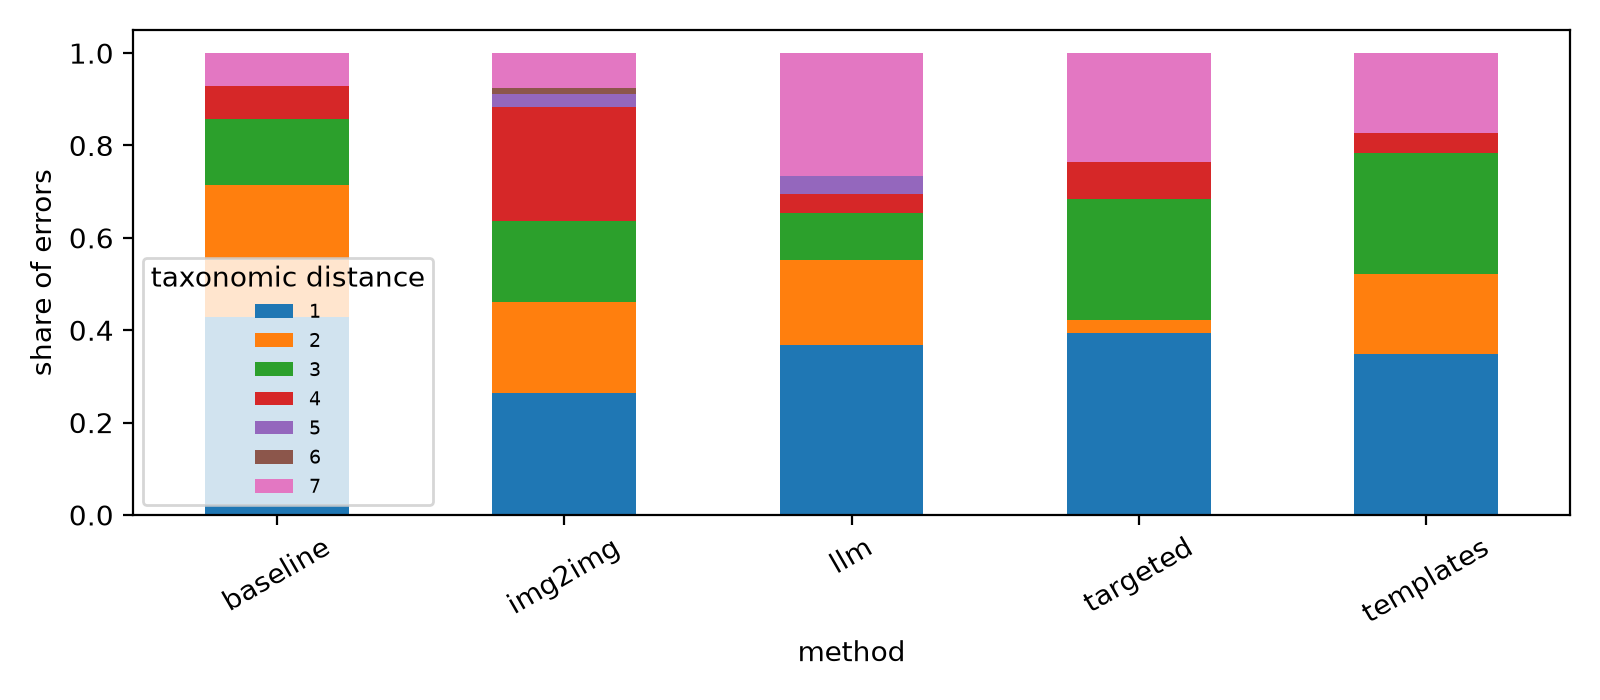
\includegraphics[width=\columnwidth]{../results/figures/taxo_distance.png}
\caption{Taxonomic distance of the errors (1 = same genus, 7 = another kingdom).}\label{fig:taxo}
\end{figure}

\subsection{Post-training}
\todo{DDPO training curves (reward, train ASR, approx. KL) from checkpoints/ddpo/train_log.csv; RAFT vs DDPO vs
best-of-N on split B; LPIPS diversity. The ablation without fidelity: reward hacking examples (figure) and its
faithful rate.}

\subsection{Transfer}
\begin{figure}[t]\centering
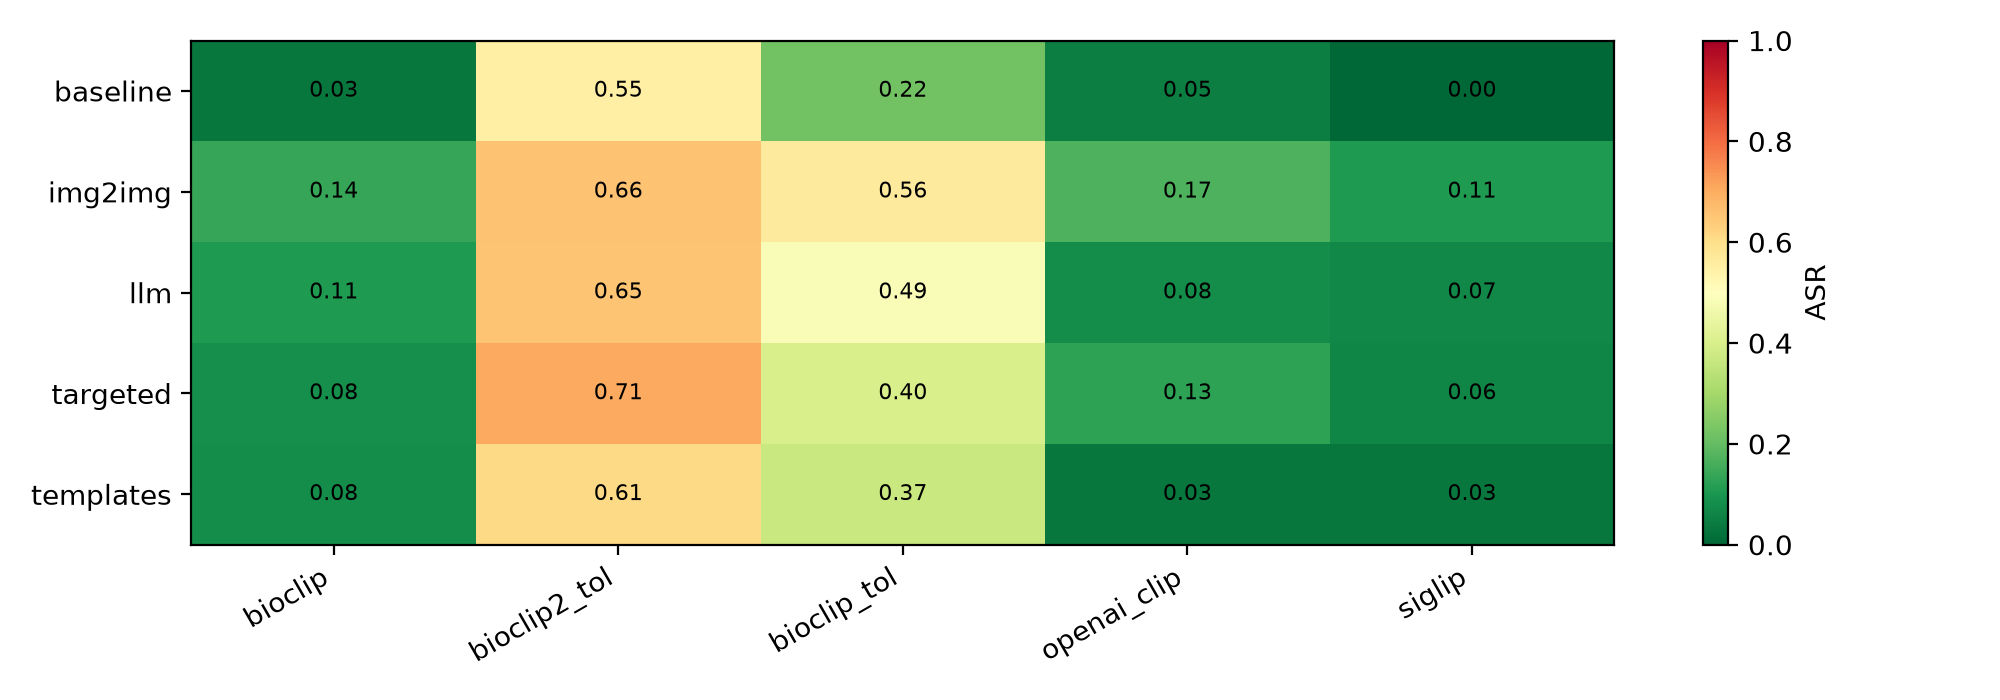
\includegraphics[width=\columnwidth]{../results/figures/transfer_heatmap.png}
\caption{ASR of the same images against other classifiers.}\label{fig:transfer}
\end{figure}
\todo{Do attacks transfer to BioCLIP-2 (the reward oracle, so a biased number), to generic CLIP and SigLIP?}

\subsection{Speed and early rejection}
\begin{table}[t]\centering\small
\caption{Sampling modes: cost and quality.}\label{tab:speed}
\resizebox{\columnwidth}{!}{\input{../results/tables/speed.tex}}
\end{table}
\todo{Table~\ref{tab:speed}: speed-up and quality loss per mode; faithful attacks per GPU-hour. Early rejection:
Spearman correlation between preview and final reward (figures/early_correlation.png), ASR of bon vs bon\_early at
their respective cost. VAE vs TAESD: PSNR and top-1 agreement (outputs/vae/vae\_fidelity.csv).}

\subsection{Why BioCLIP fails}
\todo{t-SNE (figures/tsne\_*.png), layer-wise drift of real vs attacked photos (figures/layer\_drift.png), saliency
examples (figures/saliency\_*.png), confident errors and entropy.}
